Spamiętanie wszystkich skrótów klawiaturowych może być ciężkie, zwłaszcza gdy mamy do czynienia z programami, które mają ich wiele do dyspozycji. Często też niektóre programy nie posiadają przycisków w oknie programu lub skrótów do pewnych funkcji, które to są zaszyte gdzieś głęboko w którymś z przycisków na pasku menu. Często jest tak, że pamiętamy nazwę funkcji, ale już nie bardzo miejsce, w którym się ona znajduje. I to z pomocą przychodzi HUD (Heads-up Display).

HUD jest silnie zintegrowanym narzędziem, które przy wykorzystaniu klawiatury pozwala dotrzeć do nie tylko najczęściej wykorzystywanych funkcji programu, ale również tych, o których często zapominamy gdyż są zaszytych gdzieś głęboko. Przykładowe wykorzystanie HUDa do skopiowania pliku:
\begin{center}
	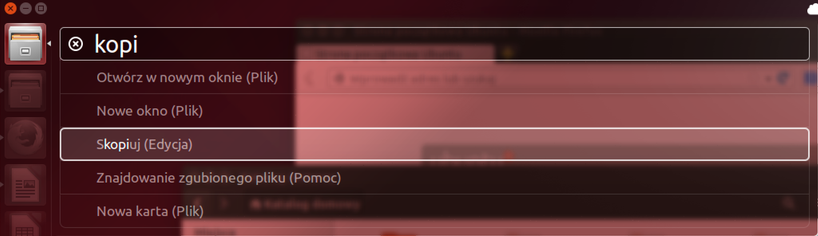
\includegraphics[scale=0.5]{images/unity_hud1.png}
\end{center}

Inny przykład. Powiedzmy, że tworzymy dokument w programie OpenOffice Writer i potrzebujemy wstawić obiekt formułę. Dla osoby, która z programu korzysta rzadko, znalezienie tej funkcji może zająć dłuższą chwilę. Wykorzystując w tym celu HUD, jest to kwestia wpisania w jego oknie słowa „formuła” i wybraniu odpowiedniej opcji w oknie wyników wyszukiwania:
\begin{center}
	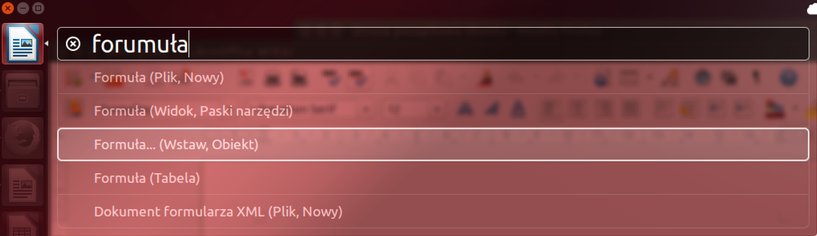
\includegraphics[scale=0.5]{images/unity_hud2.png}
\end{center}
\clearpage